\section{Omdrejningssensor - Måling af farten}
\label{fartmål}
I dette afsnit beskrives hvordan en omdrejningssensor udnyttes til at beregne hastigheden bilen kører med. Der vil både blive beskrevet hardwaren til sensoren, samt hvordan den softwaremæssigt bruger sensoren. Farten bliver brugt til beregne bremselængden, og køre med konstant hastighed, som er beskrevet i afsnit \ref{bremse} og \ref{sving}. \\

\subsection{Fart Hardware - TCST1230}
\label{fartmål_hardware}
Vi benytter TCST1230, som er en transmitiv optisk sensor, til at lave en fotogate. Sensoren består af en fotocelle og en vifte med et blad på. Hjulet med vifterne sidder på motorens aksle og hver gang akslen drejer en omgang vil den bryde fotosensorens lys en gang. Hver gang lyset brydes fås en puls fra fotosensoren, som sendes videre til microcontrolleren. Dette er illustreret i figur \ref{wheelspeed3D}.

\begin{figure}[h!]
\center
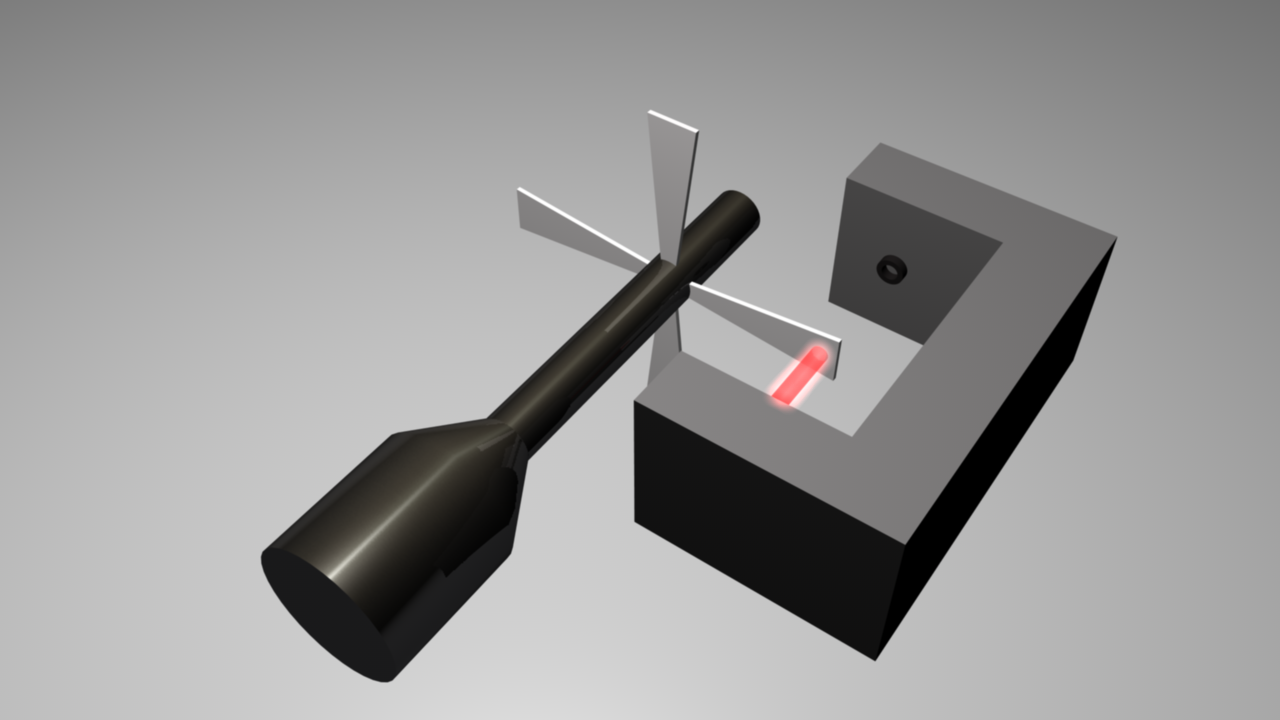
\includegraphics[scale=0.2]{./Graphics/Wheelspeed_D}
\caption{3D model af sensoren}
\label{wheelspeed3D}
\end{figure}

Efter test viste det sig at sensoren havde brug for en højre opløsning. Dette opnås ved at tilføje flere blade til viften så fås flere pulser pr. omdrejning. Der er således nu fire blade på viften, hvilket giver os fire pulser pr. aksel omdrejning. Dette svarer til 16,8 pulser pr. hjulomdrejning. \\
Se afsnit \ref{beregn_gear} for udregningen af gearingen. \\
Fire vifter giver en opløsning der er fire gange bedre, end kun at have en vifte. \\
For bedre opløsning kunne der sættes flere vifter på, men kommer der for mange vifter på, vil det dog blive svært for sensoren at aflæse vifterne. Dette skyldes at mellemrummet til sidst vil blive meget småt. Jo flere vifter der tilføjes, jo sværere bliver det også at bygge ringen med vifterne. \\

I dette tilfælde anvendes en ring med fire vifter da det kunne laves forholdsvis let, og det giver en opløsning, der er høj nok til hvad der ønskes. Ved blot en vifte kørte hjulet 2cm per omdrejning. Da hjulet kører 0,2381 omgange pr. motoromdrejning, kan længden bilen kører, mellem hver puls udregnes ved at multiplicere hjulomdrejninger med hjulets omkreds:
\begin{align*}
0,2381*8,5cm = 2,02 cm
\end{align*}
Dette er ikke ret præcist da længden og farten kun af aflæses i intervaller af 2cm. Ved fire vifter kører bilen pr. puls:
\begin{align*}
(\frac{0,2381}{4})* 8,5cm = 0,51cm
\end{align*}
Dette er markant bedre da den nu kun kører 0,51cm før den får en puls hvor den udregner længde og hastighed. Så der fås flere mindre intervaller der kan tjekkes og reageres på. \\ 

Som det kan ses på tegningen af kredsløbet i figur \ref{wheelspeedTegning} er der sat nogle modstande og en kondensator på sensorens kredsløb. \\

\begin{figure}[h!]
\center
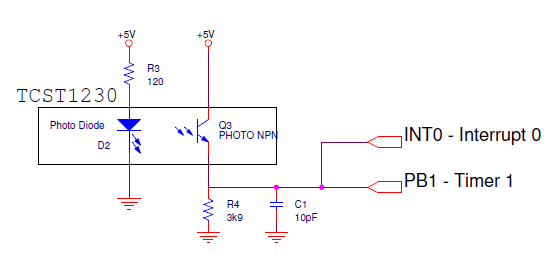
\includegraphics[scale=0.75]{./Graphics/TCST1230}
\caption{Kredsløbet til TCST1230 Sensoren}
\label{wheelspeedTegning}
\end{figure}

Modstanden R3 i figur \ref{wheelspeedTegning} er der for at strømmen gennem dioden, D2, ikke bliver større end dioden kan tåle. Dioden kan kun klare 30mA ifølge databladet\footnote{Se udsnit af datablad for TCST1230 i bilag \ref{TCST1230}}.\\

Modstanden R4 virker som en pulldown\footnote{Se ordliste \ref{ordliste}} modstand der sørger for at holde signalet lavt, når fototransistoren ikke modtager lys. \\

Kondensatoren C1 benyttes til at sortere små signaler fra. Hvis signalet ”hopper” frem og tilbage ved en overgang fra logisk lavt til logisk højt, vil kondensatoren tage de små hurtige skift og sortere dem fra. På denne måde fjernes en del af støjen.  
Ud fra Ohms lov og databladet\footnote{Se udsnit af datablad for TCST1230 i bilag \ref{TCST1230}} er modstandene bestemt, så microcontrolleren opfanger signalerne fra sensoren som højt og lavt. \\


\subsection{Fart Software}
\label{fartmål_software}
Sensorens output er sat på ”PB1” og ”PD3”\footnote{PB1 og PD3 er indgange på microcontrolleren}, som går til ”Timer1” og ”INT0”\footnote{INT0 er en interrupt indgang på microcontrolleren} i microcontrolleren. Hver gang den får en puls  bliver timeren og interruptet triggeret. Timeren bliver benyttet til at finde længden bilen har kørt. Dette er beskrevet i afsnit \ref{afstandmaal}. \\

Interruptet benyttes sammen med Timer0 til at finde farten. Timer0 er sat op så den inkrementer hvert 0,000016 sekund. Hvilket svarer til den inkrementerer hvert 16. mikrosekund. Dette er sat ved at bruge en prescale på 256. Da klokfrekvensen på microcontrolleren er 16MHz udregnes det således:
\begin{align*}
\frac{256}{16 000 000Hz} = 0,000016 s = 16 \mu s 
\end{align*}

Dette bruges til at finde periodetiden, som benyttes til at udtrykke farten. Et overflow vil kun forekomme hvis noget går galt og bilen står helt stille, eller kører under 1,2\(m/s\). Hvis der er overflow i Timer0, kaldes et andet interrupt, der sætter en konstant hastighed. \\

Flowdiagrammet i figur \ref{fart_chart} viser processen hver gang interruptet bliver kaldt. Hvilket sker hver gang sensoren sender en puls. \\

\begin{figure}[h!]
\center
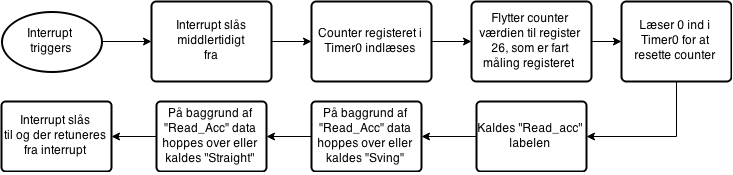
\includegraphics[scale=0.65]{./Graphics/fart_chart}
\caption{Flowchart af softwaren til måling af farten}
\label{fart_chart}
\end{figure}

Der slås først interrupts fra globalt, for at dette interrupt ikke bliver afbrudt af et andet interrupt. Herefter indlæses den værdi tælleren er nået til. Denne værdi gemmes i vores ”målt fart” register. Derefter nulstilles Timer0. På den måde får vi hvor mange gange der er gået 16 mikrosekunder på 1 puls. F.eks. hvis der går 80 optællinger mellem timer puls, så har bilen farten: \(~4 m/s\). \\
Dette kan ses i lookup table i afsnit \ref{lookup}.

Inden interruptet sluttes læses accelerometeret, som er nærmere beskrevet i afsnit \ref{svingsensor}. \\

Til sidst slås interrupts til igen og koden fortsætter hvor den blev afbrudt af interruptet.  
